\section{Results}
\begin{table}[b]
  \centering
  \begin{tabular}{|l|c|c|c|c|c|}
    \hline
    examples 		& cloth 	& act- 	& anim	& sim 		& control \\
                    & triangles & 	ions& time 	& time 		& time \\
    \hline
    jacket 			& 23.2k  	& 10	& 18s 	& 30h23m	&  14m  \\
    jacket (low res)& 2.7k		& 10	& 18s	& 2h58m		& 1m \\
    shorts (sitting) 	& 14.9k 	& 10	& 16s 	&  8h41m 	& 4m \\
    shorts (standing)	& 14.9k 	& 10	& 15s	&  7h52m	& 3m \\
    vest 			& 6.57k		& 14	& 13s	&  3h53m	& 1m   \\
    robe 			& 31.7k 	& 11	& 14s	& 20h40m	& 19m  \\
    \hline
  \end{tabular}
  \caption{Parameters and performance of the examples. cloth triangles: the number of elements in cloth simulation. Actions: number of actions. Anim time: wall clock time (in seconds) of the dressing animation. Sim and control times are the total times for the cloth simulation and our control functions respectively.}
  \label{table:data}
\end{table}


In this section we describe the results of our system. We chose four different types of garments from the Berkeley Garment Library, edited them to meet our needs, and put them on the character using different styles. \new{All motion capture sequences used in the examples were acted out from memory, without real cloth garments.} Please watch the accompanying video for the dressing animations. Our system was implemented in C++. We used DART \cite{Liu:2012:STM} for human character modeling and ARCSim \cite{Narain:2012:AAR} for cloth simulation. We used a denim material profile with 3-4x thickening to simulate layered clothing articles. The examples were run on a desktop workstation with a 4-core 3.7 GHz CPU and 8 GB of memory. The typical running time of a dressing example is several hours to a day. The cloth simulation is the most time-consuming part and takes significantly longer than control. \new{We solve the Inverse Kinematics optimization with SNOPT, which uses a sequential quadratic program solver.} The parameters and performance data of our examples are summarized in Table
 \ref{table:data}.


\paragraph{Jacket.} Figure~\ref{fig:jacket} shows a character putting on a
jacket using a common style: Put the left arm in its sleeve, swing the right arm to the back, find the hanging sleeve, and stretch the arm into it. The reference human motion for this style is made up of six keyframes. As shown in the video, dressing by directly playing back the reference motion without any feedback control fails to put on even the first sleeve. After gripping the collar of the cloth, our system first tracks the reference motion to a particular keyframe and then performs an alignment action. The character aligns his left hand with the corresponding armhole. Once the alignment is successful, the traversal action is executed. The character uses his right hand to drag the cloth up the length of the left arm. At the end of traversal, the right hand reaches the shoulder and releases the cloth. The character then swings his right arm to the back by tracking the reference motion. The second alignment phase begins when the character's right hand starts to search for the opening of the sleeve. This alignment phase is more challenging because the target armhole is completely occluded by multiple layers of cloth. The alignment action gradually finds better intermediate goals that are closer to the target feature and guides the hand to wiggle through the cloth folds towards the goal. 

In the jacket example we observed interesting emergent behavior, such as a natural exploratory gesture that is often used by humans to sort out the tangled cloth in dressing. Furthermore, the hand operates within a tight space between the pelvis and the hanging cloth during alignment. Without the collision-free IK, the hand or arm would penetrate the torso before aligning with the armhole. After the alignment, the character uses the traversal action to stretch the right arm into the sleeve and then tracks the reference motion until the jacket is completely on the body. 

A common challenge in cloth simulation is that the simulation may produce
drastically different motions if the resolution of the cloth changes. To
test the robustness of our system, we used the same actions to put on a
low resolution jacket with approximately 10x fewer triangles. Our system
was able to automatically adapt to the change in resolution and the
resulting differences in cloth motion without any manual tuning. Note that
the more coarse resolution cloth has fewer wrinkles and folds.  A
consequence of this is that the lower resolution jacket has a less occluded
armhole, so the right hand alignment phase is shorter in this sequence.

\paragraph{Vest.} We simulated putting on a vest in a more dynamic style (Figure~\ref{fig:vest}). We chose this example to demonstrate that using a small set of primitive actions, our system is able to put on a garment in a different style by using a different reference motion. Tracking the motion captured reference, the character swings the vest around his neck, then aligns the left hand with the corresponding armhole while the vest is swinging in mid-air. This alignment shows that our feedback control is robust and able to align not only with a target feature that is occluded by layers of cloth, but also with one that is moving quickly. Once the first arm is dressed, the right hand is aligned with the second armhole and stretches into it. 

\begin{figure*}[!t]
  \centering
  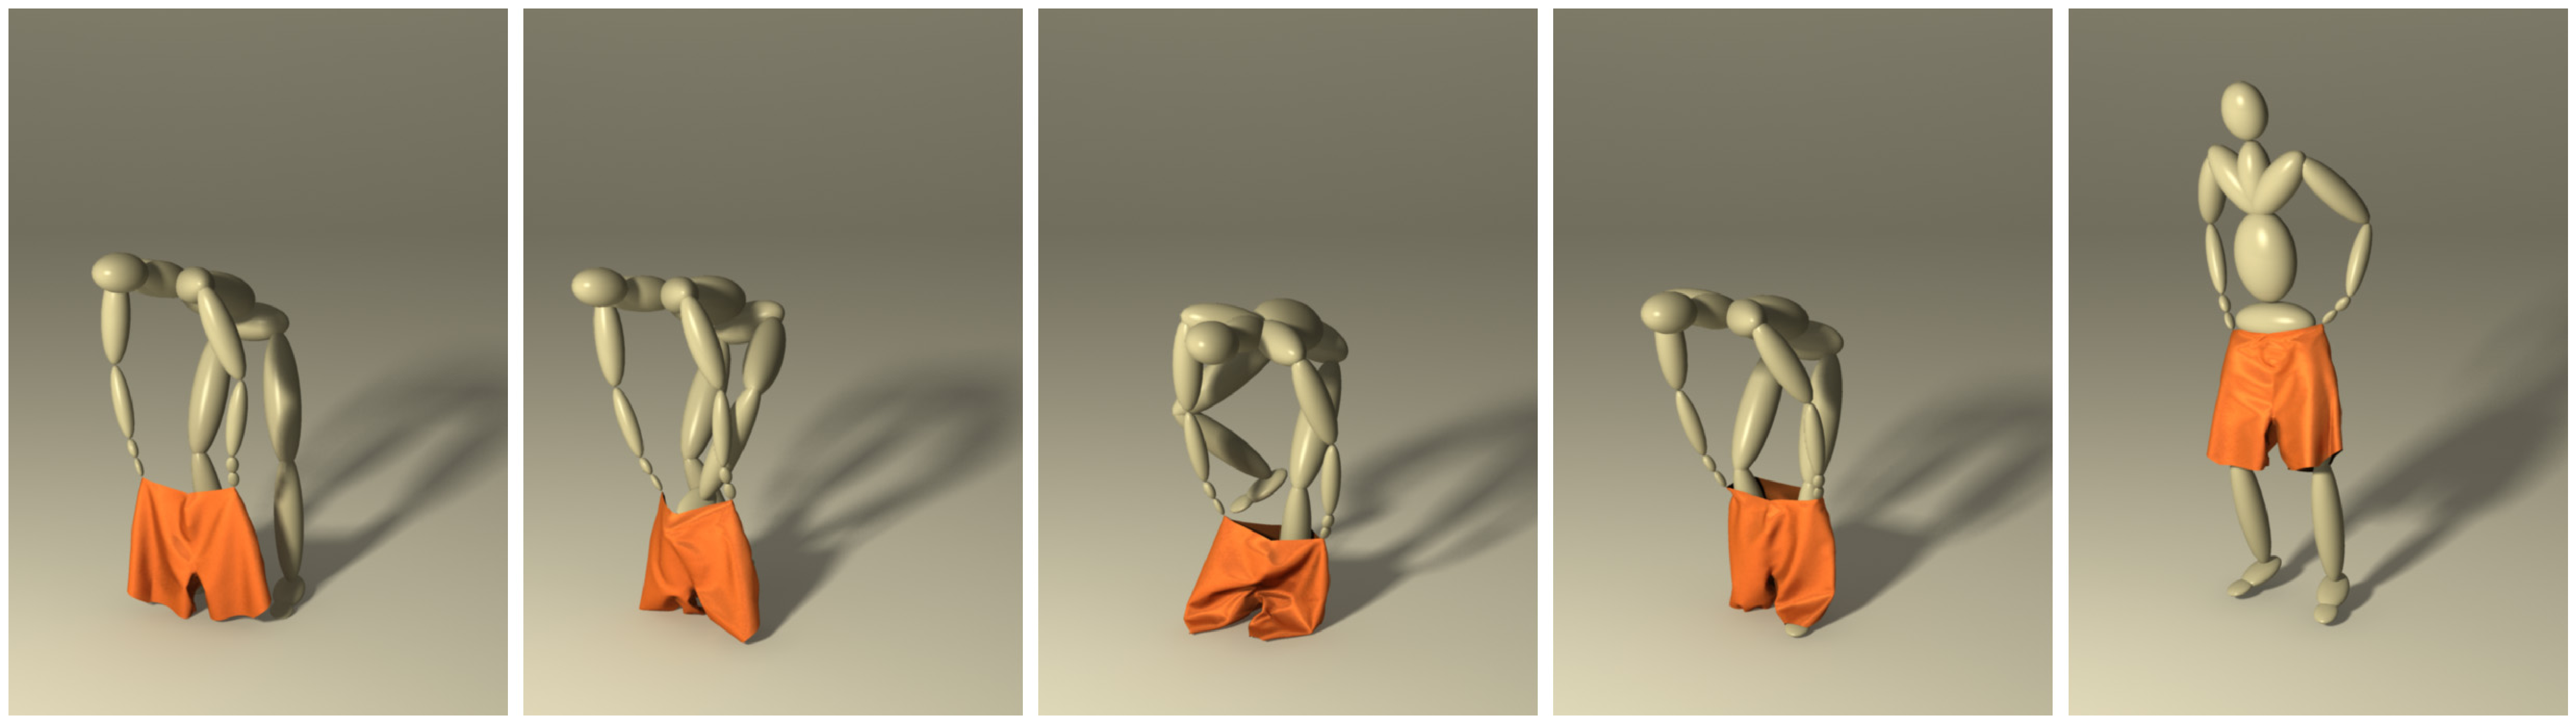
\includegraphics[width=\textwidth]{images/shortsStanding}
  \caption{A character puts on a pair of shorts in a standing pose.}
  \label{fig:shorts2}
\end{figure*}

\begin{figure*}[!t]
  \centering
  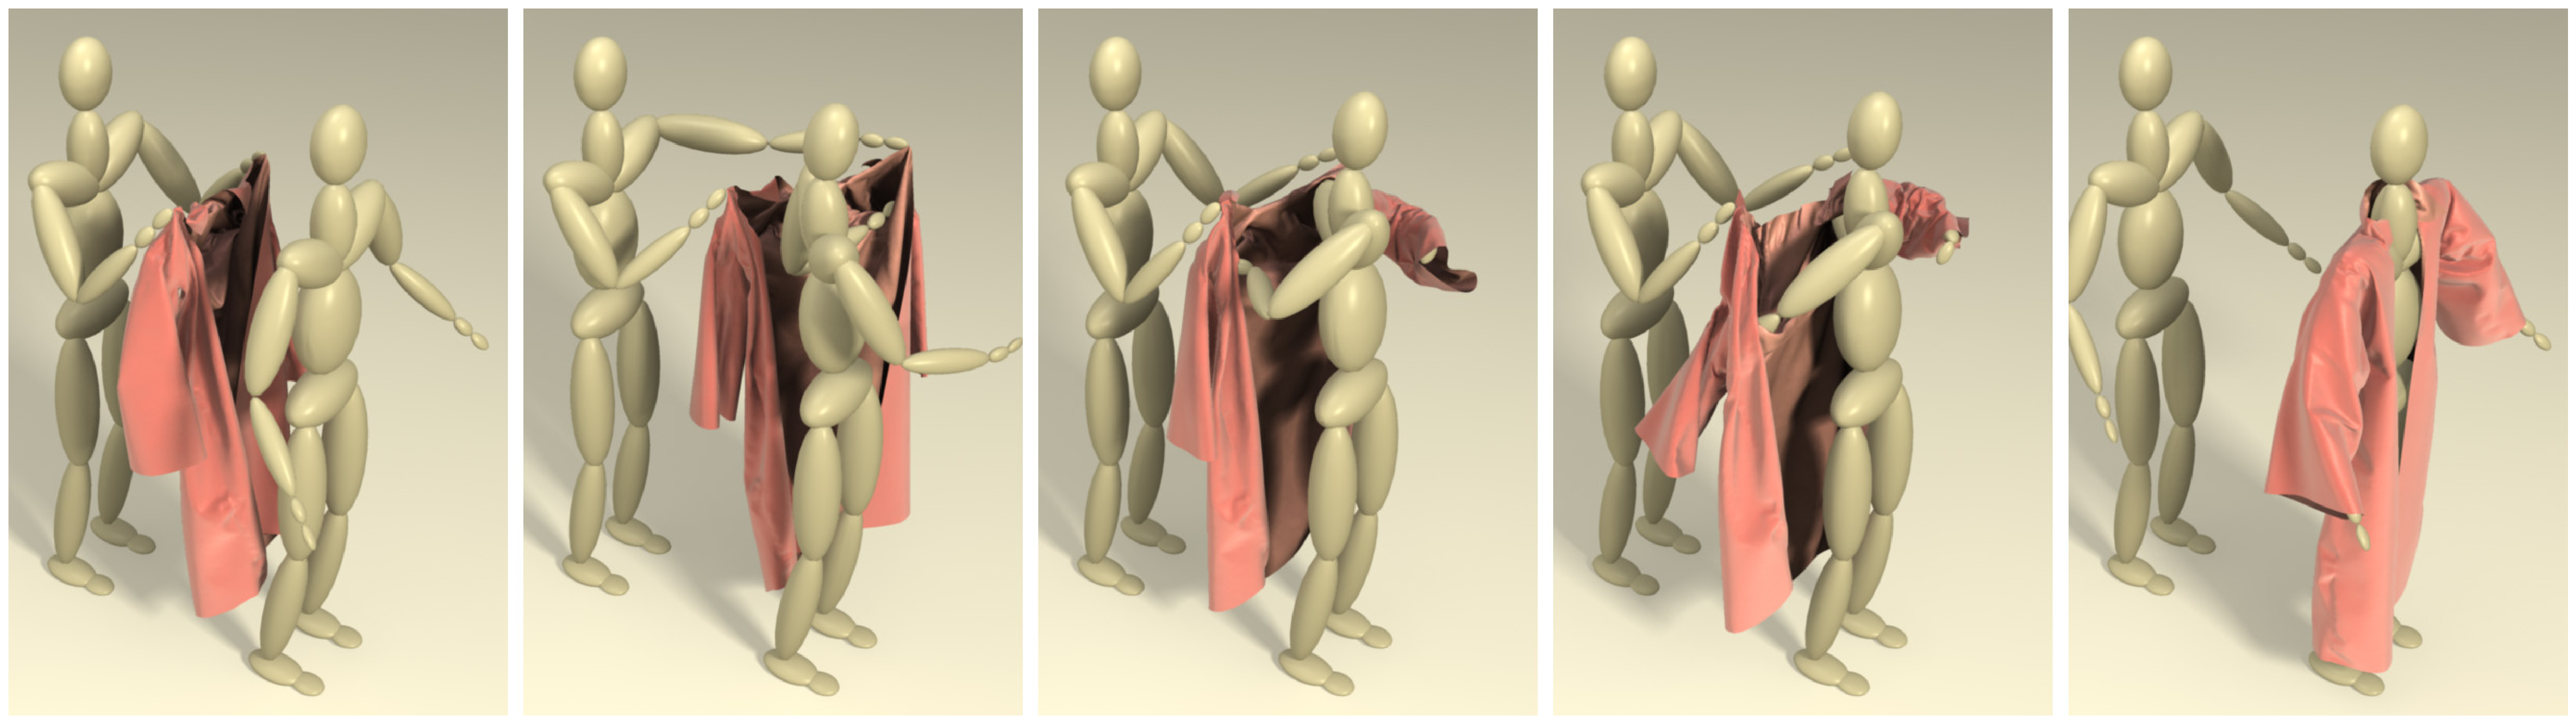
\includegraphics[width=\textwidth]{images/robe}
  \caption{A character puts on a robe with the help from another character.}
  \label{fig:robe}
\end{figure*}

\paragraph{Shorts.} Figure~\ref{fig:shorts1} demonstrates a character that
is putting on a pair of shorts in a sitting position. We used a motion
capture sequence as the reference motion in this example. The character
grips the waistband and leans forward by tracking the reference motion. He
first aligns his left foot with the waistband and then aligns it with the
bottom of the shorts' left leg. Similar alignment actions are applied to
the right foot. Once both feet are aligned with the desired features, the
character follows the reference motion to stand up and pull up the shorts.
The accompanying video shows that without the feedback control, the
character fails to put the feet into the shorts and ends up not wearing
the pants.

We also tested the generality of our system by using a different reference motion, in which we mocaped a person that is putting on a pair of shorts in a standing position. Despite the different style, we were able to reuse the action queue from the sitting shorts and successfully dress the lower body of the character (Figure \ref{fig:shorts2}).

\paragraph{Robe.} To show that our system can be used outside of the realm of self-dressing, we applied our method to an assisted dressing scene in which one character aids another in putting on a robe (Figure \ref{fig:robe}). The reference motion for this scene consists of five keyframes. First, the dressing character tracks the reference motion, twisting to the left and aligning his left hand with the armhole. After he straightens his arm into the sleeve, the assistant releases the cloth from his left hand. Dressing the second arm is similarly performed with both characters tracking to a pre-alignment position whereupon the dressing character aligns and straightens his arm and the assistant releases the sleeve. Note that in this example, the dressing control is only performed on the dressing character while the motion of the assistant is pre-scripted. It would be interesting future work to simulate and control both characters in an assisted dressing task.
